% !TeX program = xelatex
\documentclass[a4paper,12pt]{article}
\usepackage{tikz}
\usepackage[bottom]{footmisc}
\usepackage{subcaption}
\usepackage{listings}
\usepackage{xcolor}
\usepackage[colorlinks = true,
linkcolor = blue,
urlcolor  = blue,
citecolor = blue,
anchorcolor = blue]{hyperref}
\usepackage{fullpage,amsmath,hyperref,color,clrscode,amsfonts,graphicx,textcomp}
\usepackage{tabularx}
\usepackage{adjustbox}
\usepackage{setspace}
\usepackage{upgreek}
\usepackage{amsmath}
\usepackage{amssymb}
\usepackage{tikz}
\usepackage[inline]{enumitem}
\usepackage{pgfplots}
\usetikzlibrary{calc}
\newcommand{\drawaline}[4]{
	\draw [extended line=1cm,stealth-stealth] (#1,#2)--(#3,#4);
}
\usepackage{float}
\usetikzlibrary {positioning}
%\usepackage {xcolor}
%\definecolor {processblue}{cmyk}{0.96,0,0,0}
\definecolor {processblue}{cmyk}{1,1,1,0}
\usetikzlibrary{automata,arrows.meta}
\usepackage{hyperref}
\usepackage{multirow}
\usepackage{graphicx}
\usepackage{neuralnetwork}
\usepackage{tkz-graph}
\hypersetup{
	colorlinks=true,
	linkcolor=red,
	filecolor=blue,      
	urlcolor=magenta,
}


\usetikzlibrary{arrows, positioning}
\usepackage{xepersian}

\definecolor{codegreen}{rgb}{0,0.6,0}
\definecolor{codegray}{rgb}{0.5,0.5,0.5}
\definecolor{codepurple}{rgb}{0.58,0,0.82}
\definecolor{backcolour}{rgb}{0.95,0.95,0.95}

\lstdefinestyle{mystyle}{
	backgroundcolor=\color{backcolour},   
	commentstyle=\color{codegreen},
	keywordstyle=\color{magenta},
	numberstyle=\tiny\color{codegray},
	stringstyle=\color{codepurple},
	basicstyle=\ttfamily\footnotesize,
	breakatwhitespace=false,         
	breaklines=true,                 
	captionpos=b,                    
	keepspaces=true,                 
	numbers=left,                    
	numbersep=5pt,                  
	showspaces=false,                
	showstringspaces=false,
	showtabs=false,                  
	tabsize=2
}

\lstset{style=mystyle}

\settextfont[Path="./fonts/",Scale=0.99 , BoldFont = XB Zar bold.ttf]{XB Zar.ttf}
\setlatintextfont[Path="./fonts/"]{Times New Roman.ttf}

\addtolength{\textwidth}{0.2in}
\addtolength{\oddsidemargin}{-0.1in}
\addtolength{\evensidemargin}{-0.1in}

\addtolength{\textheight}{0.5in}
\addtolength{\topmargin}{-0.25in}
\defpersianfont\iranic[Path="./fonts/",Scale=1]{XB Zar.ttf} 	
\newcommand{\IP}{\mathbb{P}}

\makeatletter
\def\LTRfootnote{\@ifnextchar[\@xLTRfootnote{\stepcounter\@mpfn
		\protected@xdef\@thefnmark{\persianfont\thempfn}%
		\@footnotemark\@LTRfootnotetext}}
\makeatother	
\setdigitfont[Path="./fonts/",Scale=1]{XB Zar.ttf} 
\setmathdigitfont[Path="./fonts/",Scale=1]{XB Zar.ttf} 
\usepackage{assets/template}
\newcommand{\hidesolutions}{}

\begin{document}
{\centering به نام زیباترین}\\
	\def\ci{\perp\!\!\!\perp}

	% header{<Assignment-Number>}{<Assignment-Title>}{<Deadline-Date>}{<Gathered-by>}{<Supervised-by>}
	\header
		{6 دی ۱۴۰۳}
		{آزمون میان‌ترم دوم}
		{زمان:  3  ساعت}
		{امیرمهدی میقانی - علی رحیمی اکبر - پیام تائبی}{}
	\begin{itemize}
	\small
	\setlength\itemsep{0.05em}

\end{itemize}
\vspace{-3mm}
نام و نام خانوادگی: \hspace{8cm} شماره دانشجویی:

\hrule
\vspace{2mm}
لطفا پاسخ هر سوال را زیر آن بنویسید. بالای \textbf{هر برگه نام و شماره دانشجویی} خود را حتما قید کنید. در پایان آزمون، برگه‌ی سوال‌های مختلف را از هم جدا کنید و هر برگه را در دسته‌ی مربوط به خود قرار دهید.
این آزمون از 110 نمره است و نمره کامل 100 است. توجه کنید نمره‌ی بالای 100 امتیازی نخواهد داشت.



\vspace{0.5cm}
\textbf{اصلی}

در یک شرکت بزرگ کاریابی کار می‌کنید. هر فرد یک پروفایل دارد که بعضی ویژگی‌های آن (نظیر سن، آخرین حقوق) عدد پیوسته و بعضی ویژگی‌های دیگر (نظیر رشته‌ی تحصیلی) Categorical است. 
همچنین بعضی از ویژگی‌ها (نظیر آشنایی با هریک از زبان‌های برنامه‌نویسی) به صورت صفر و یک درج شده است. 

\begin{enumerate}
\item می‌خواهید برای هر کاربر جدید که پروفایل خود را تکمیل کرده‌است، یک مبلغ حقوق تخمین بزنید. از چه الگوریتمی استفاده می‌کنید؟ چه تغییری روی ویژگی‌ها می‌دهید؟ برای هریک از ویژگی‌ها از چه پیش‌پردازشی استفاده می‌کنید؟ جزئیات را توضیح دهید.
\vspace{5cm}
\item
حال می‌خواهید داده‌های این شرکت را به صورت یک نمودار نمایش دهید. برای این کار تصمیم دارید از تحلیل مولفه‌های اصلی (PCA) استفاده کنید.
آیا به نظر شما تغییر مقیاس ویژگی‌ها لازم است؟ اگر بله، چرا؟ و چطور این کار را انجام می‌دهید؟ اگر خیر، دلیل‌ شما چیست؟
\vspace{5cm}
\item
فرض کنید ماتریس کوواریانس زیر را داشته باشید. چطور از روی آن مولفه‌های اصلی را مشخص می‌کنید؟ محاسبات خود را بنویسید.
{\latin
\centering
$C=$\begin{bmatrix}
3 & -4\\
-4 & 3
\end{bmatrix}
}
\vspace{5cm}
\item
فرض کنید می‌خواهید با PCA ابعاد داده‌هاهای شرکت را با بردن آن‌ها فضای جدیدی کاهش دهید که عمده‌ی اطلاعات حفظ شود. چطور تعداد بعدهای فضای جدید را مشخص می‌کنید؟
\vspace{6cm}
\item
ثابت کنید تصویرکردن داده‌ها توسط بردارویژه‌‌ی با بزرگ‌ترین مقدار ویژه‌ی ماتریس کوواریانس، واریانس داده‌های تصویرشده را بیشینه می‌کند.
\vspace{6cm}
\item
به دل‌خواه یک مساله‌ی زیبای یادگیری ماشین بنویسید و آن را حل کنید. نمره‌ی این بخش به زیبایی و منحصر به فرد بودن مساله‌ و درستی راه‌حل شما اختصاص می‌یابد.

\end{enumerate}

\pagebreak
\vspace{1cm}

پاسخ سوال اول) گزینه‌های الف و ب

\vspace{1cm}

پاسخ سوال دوم) گزینه‌های الف و د




\vspace{1cm}
پاسخ سوال سوم)



الف نادرست و ب درست می‌باشد


مدل‌های خودرمز‌گذار پراکنده، بدون نیاز به regularization خاصی شامل گلوگاه اطلاعاتی می‌باشند. گزاره ب نیز تعریف این دسته از مدل‌ها می‌باشد.

\vspace{1cm}


ج درست و د درست می‌باشد




در گزاره اول، با کاهش تعداد نورون‌ها می‌توان میزان اطلاعات در مدل خودرمز‌گذار را کاهش و درنتیجه آن را به مدل خودرمزگذار ناقص تبدیل کرد. در گزاره دوم، به صورت‌کلی مدل‌های خودرمزگذار را میتوان به‌عنوان یک ابزار کاهش ابعاد داده ( reduction dimensionality ) درنظر گرفت که برای این امر، مدل ابرصفحه‌هایی را برای تصویر کردن داده به ابعاد پایین‌تر را یاد می‌گیرد.

\vspace{1cm}

ه درست  و درست می‌باشد




این مدل برای از بین بردن نیز در داده ورودی استفاده می‌شود، درنتیجه تابع هزینه زمان آموزش این مدل سعی می‌کند تفاوت میان نسخه اصلی داده ورودی و بازسازی داده براساس نسخه نویزی آن را کاهش دهد. خروجی بخش رمز‌گذار مدل (و ورودی بخش رمز‌گشا) ویژگی‌های استخراج‌شده از داده توسط مدل می‌باشند.
\pagebreak
\hrule
% % نام و نام خانوادگی: \hspace{8cm} شماره دانشجویی:
% % \hrule
% % \vspace{0.5cm}
% \textbf{سوال چهارگزینه ای(9 نمره)}



در هریک از سوال‌های زیر، با انتخاب گزینه مناسب گزاره‌های درست را انتخاب کنید.

\vspace{0.5cm}
۱.

الف) در مدل‌های خودرمز‌گذار پراکنده \footnote{autoncoder Sparse} ایجاد تعداد نورون‌ها در لایه نهان مدل \footnote{layer Hidden} باعث ایجاد گلوگاه اطلاعاتی \footnote{bottleneck Information} می‌شود.

\vspace{0.25cm}
ب) ایده کلی در مدل خودرمز‌گذار پراکنده این است که روند رمز‌گذاری و رمزگشایی تنها با فعال نگه‌داشتن تعداد کمی از نورون‌ها صورت بگیرد

\vspace{0.5cm}
۱)  الف درست و ب نادرست است.

\vspace{0.25cm}
۲) هردو نادرست هستند.

\vspace{0.25cm}
۳) هردو درست هستند.

\vspace{0.25cm}
۴)  الف نادرست و ب درست است.

\vspace{0.5cm}
۲.

الف) یک راه برای ایجاد مدل خودرمز‌گذار ناقص \footnote{autoencoder Sparse} این است که تعداد نورون‌های موجود در لایه‌های نهان \footnote{layers Hidden} را کاهش دهیم.

\vspace{0.25cm}
ب) مدل‌های خودرمزگذار قادر به یادگیری منیفولد‌های \footnote{Manifold} غیرخطی می‌باشند.

\vspace{0.5cm}
۱) الف درست و ب نادرست است.

\vspace{0.25cm}
۲) هردو نادرست هستند.

\vspace{0.25cm}
۳) هردو درست هستند.

\vspace{0.25cm}
۴) الف نادرست و ب درست است.

\vspace{0.5cm}
۳.

الف) در مدل خودرمزگذار بدون نویز \footnote{autoencoder Denoising}، تابع هزینه میان نسخه اصلی ورودی و بازسازی آن براساس نسخه نویزی آن، محاسبه می‌شود.

\vspace{0.25cm}
ب) از مدل خودرمزگذار بدون نویز میتوان به‌عنوان ابزاری برای استخراج ویژگی استفاده کرد.

\vspace{0.5cm}
۱) الف درست و ب نادرست است.

\vspace{0.25cm}
۲) هردو نادرست هستند.

\vspace{0.25cm}
۳) هردو درست هستند.

\vspace{0.25cm}
۴) الف نادرست و ب درست است.

% 
\vspace{5cm}
پاسخ سوال ۱. گزینه ۴:‌الف نادرست و ب درست می‌باشد.

مدل‌های خودرمز‌گذار پراکنده، بدون نیاز به regularization خاصی شامل گلوگاه اطلاعاتی می‌باشند. گزاره ب نیز تعریف این دسته از مدل‌ها می‌باشد.

\vspace{1cm}

پاسخ سوال ۲. گزینه ۳:‌ هردو گزاره درست هستند.

در گزاره اول، با کاهش تعداد نورون‌ها می‌توان میزان اطلاعات در مدل خودرمز‌گذار را کاهش و درنتیجه آن را به مدل خودرمزگذار ناقص تبدیل کرد. در گزاره دوم، به صورت‌کلی مدل‌های خودرمزگذار را میتوان به‌عنوان یک ابزار کاهش ابعاد داده ( reduction dimensionality ) درنظر گرفت که برای این امر، مدل ابرصفحه‌هایی را برای تصویر کردن داده به ابعاد پایین‌تر را یاد می‌گیرد.

\vspace{1cm}

پاسخ سوال ۳. گزینه ۳: هردو گزاره درست هستند.

این مدل برای از بین بردن نیز در داده ورودی استفاده می‌شود، درنتیجه تابع هزینه زمان آموزش این مدل سعی می‌کند تفاوت میان نسخه اصلی داده ورودی و بازسازی داده براساس نسخه نویزی آن را کاهش دهد. خروجی بخش رمز‌گذار مدل (و ورودی بخش رمز‌گشا) ویژگی‌های استخراج‌شده از داده توسط مدل می‌باشند.
% \pagebreak
% \hrule
نام و نام خانوادگی: \hspace{8cm} شماره دانشجویی:
\hrule
\vspace{0.5cm}


ماتریس داده زیر را در نظر  بگیرید که چهار نمونه $X_i \in R^2$ را نشان می‌دهد:

$$X= \begin{pmatrix}
 4 & 1  \\
 2& 3 \\
 5& 4 \\
 1& 0  \\
\end{pmatrix}$$

\begin{enumerate}
    \item [الف)] جهت‌های مولفه اصلی با طول واحد $X$ را محاسبه کنید و بیان کنید که اگر فقط به دنبال یک مولفه اصلی باشیم،  الگوریتم $PCA$ کدام یک را انتخاب می‌کند. 
    \item[ب)] بهترین (با حداقل خطای بازسازی) projection از $X$ را در یک زیرفضای یک بعدی با مبدا صفر پیدا کنید.
\end{enumerate}


\pagebreak
\textbf{پاسخ}
(الف) $Ausgmentation$ های مختلف یکی از جواب ها است.

(ب)
\begin{equation}
z_1 = \begin{bmatrix}
0.2&0.4&-0.5 \\
-0.3&0.1&0.2
\end{bmatrix} 
\begin{bmatrix}
1 \\
0 \\
1
\end{bmatrix} + \begin{bmatrix}
-0.4\\
0.2
\end{bmatrix} = \begin{bmatrix}
-0.7\\
0.1
\end{bmatrix}
\end{equation}

\begin{equation}
a_1=\begin{bmatrix}
0.\\
0.1
\end{bmatrix}
\end{equation}

\begin{equation}
z_2 = \begin{bmatrix}
-0.3&0.2 \\
\end{bmatrix} 
\begin{bmatrix}
0 \\
0.1
\end{bmatrix} + \begin{bmatrix}
0.1
\end{bmatrix} = 0.08
\end{equation}

\begin{equation}
    \hat{y}(i) = \frac{1}{1+\epsilon^{-0.08}}\approx 0.52
\end{equation}
\begin{equation}
    L(i) = 0.5(log0.52) \approx 0.142
\end{equation}

(ج) وزن دهی به اینکه هرکلاس چقدر در تابع ضرر مشارکت دارد می تواند به نزول گرادیان کمک کند، زیرا شبکه هنگام یادگیری از نمونه های کلاس کم تعدادتر، قدم های بزرگتری خواهد داشت.
$\alpha = 0.1$ و $\beta = 1$ بطور تقریبی، نسبت باید جایی در حدود $\beta =10 \cdot a $ باشد، اما نه خیلی بزرگ یا کوچک باشد.

(د) 

\begin{equation}
    \frac{\partial j}{\partial \hat{y}} = -\frac{1}{m} \sum_{i} \delta_1^{(i)}    
\end{equation}
که در آن :
\begin{equation}
    \delta_1^{(i)} = a \cdot y^{(i)}/ \hat{y}^{(i)} - \beta \cdot (1-y^{(i)})/(1-\hat{y}^{(i)})
\end{equation}

\begin{equation}
    \frac{\partial \hat{y}^{(i)}}{\partial z_2} = \delta_2 = \sigma(z_2)(1-\sigma(z_2))
\end{equation}

\begin{equation}
    \frac{\partial z_2}{\partial a_1}=\delta_3=W_2
\end{equation}
\begin{equation}
    \frac{\partial z_2}{\partial W_2}=\delta^\prime_3=a^T_1
\end{equation}
\begin{equation}
    \frac{\partial z_1}{\partial W_1}=\delta_4= 
    \begin{cases}
    0&  z_1<0\\
    1& z_1\geq 0
\end{cases}
\end{equation}
\begin{equation}
    \frac{\partial z_1}{\partial W_1}=x^{(i)T}
\end{equation}
\begin{equation}
    \frac{\partial J}{\partial W_1}=\delta_6=-\frac{1}{m} \sum_i \delta_1^{(i)}\cdot \delta_2 \cdot (\delta_3 \odot \delta_4) \cdot \delta_5
\end{equation}
\begin{equation}
    \frac{\partial J}{\partial W_2}=\delta_7=-\frac{1}{m} \sum_i \delta_1^{(i)}\cdot \delta_2 \delta^\prime_3
\end{equation}
که در آن $\delta_1^{(i)}$ و $\delta_2$ اسکالر هستند و $\delta_3 , \delta_4 \in \mathbb{R}^{D_{w1} \times 1}$ و $\delta_5 \in \mathbb{R}^{1 \times D_x}$
\begin{equation}
    W_1^{(0)} = W_1 - \eta \cdot \frac{\partial J}{\partial W_1}
\end{equation}
\begin{equation}
    W_2^{(0)} = W_2 - \eta \cdot \frac{\partial J}{\partial W_2}
\end{equation}

(ه)

\begin{equation}
    J2 = - \sum_i (\alpha \cdot (1-y^{(i)}).log(1-\hat{y}^{(i)})+\beta \cdot y^{(i)} \cdot log(\hat{y}^{(i)})) + \frac{1}{2}||W_2||_2^2+\frac{1}{2}||W_1||_2^2
\end{equation}
\begin{equation}
    J1 = - \sum_i (\alpha \cdot (1-y^{(i)}).log(1-\hat{y}^{(i)})+\beta \cdot y^{(i)} \cdot log(\hat{y}^{(i)})) + \frac{1}{2}||W_2||_1+\frac{1}{2}||W_1||_1
\end{equation}
\begin{equation}
    W_1^{(0)} = W_1 -\eta \cdot (\frac{\partial j}{\partial W_1}+2 \cdot W_1)
\end{equation}

\pagebreak
\hrule
نام و نام خانوادگی: \hspace{8cm} شماره دانشجویی:
\hrule
\vspace{0.5cm}
\textbf{خرد جمعی}

می‌دانیم که Adaboost یک دسته‌بند \(H\) را با استفاده از جمع وزن‌دار یادگیرنده‌های ضعیف \(h_t\) به صورت زیر یاد می‌گیرد:

\begin{latin}
    
\[
H(x) = \operatorname{sgn} \left( \sum_{t=1}^T \alpha_t h_t(x) \right)
\]
\end{latin}


در این سوال، ما از درخت‌های تصمیم به عنوان یادگیرنده‌های ضعیف خود استفاده می‌کنیم، که یک نقطه را به عنوان \(\{1, -1\}\) بر اساس دنباله‌ای از \lr{threshold}ها روی ویژگی‌های آن (اینجا \(x, y\)) طبقه‌بندی می‌کنند.

در سوالات زیر فرض کنید 
 که در صورت برابری امتیاز برای کلاس مثبت و منفی، خروجی دسته‌بندها به طور دلخواه تعیین می‌شود.
\vspace{-5mm}
\begin{enumerate}
\item
فرض کنید یادگیرنده‌های ضعیف ما درخت‌های تصمیم با عمق 1 هستند (\lr{Decision Stumps})، که خطای آموزشی وزن‌دار را کمینه می‌کنند. با استفاده از مجموعه داده زیر، مرز تصمیمی که توسط \(h_1\) یاد گرفته شده است را ترسیم کنید.
\vspace{-5mm}
\begin{figure}[H]
    \latin
    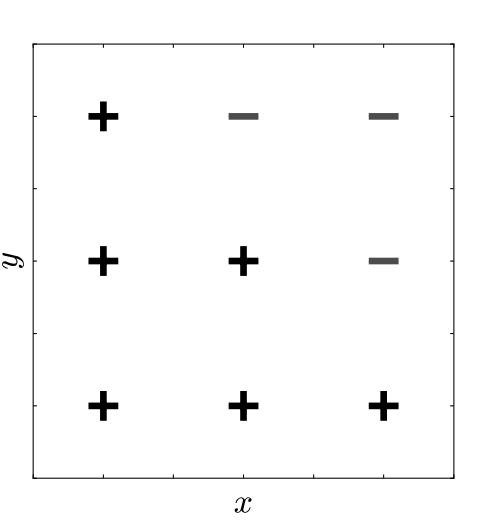
\includegraphics[width=0.28\linewidth,left]{images/2-1.png}
\end{figure}
\vspace{-5mm}
\item
 در مجموعه داده‌ی زیر، نقطه(های) با بیشترین وزن در \lr{iteration} دوم را مشخص و مرز تصمیمی که توسط \(h_2\) یاد گرفته شده است را ترسیم کنید.
 \vspace{-5mm}
\begin{figure}[H]
    \latin
    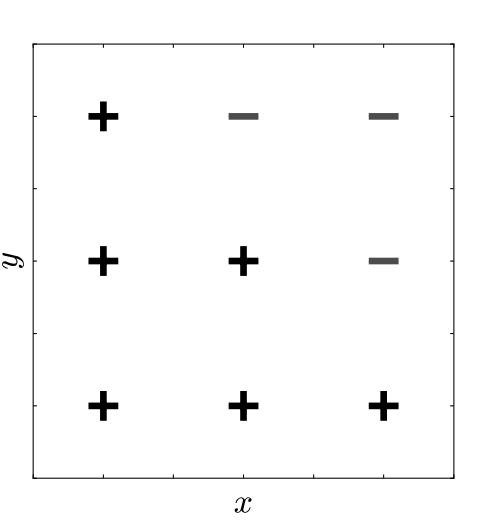
\includegraphics[width=0.28\linewidth,left]{images/2-1.png}
\end{figure}
\vspace{-5mm}
\item
در مجموعه داده‌ی زیر، مرز تصمیم \(H = \operatorname{sgn} (\alpha_1 h_1 + \alpha_2 h_2)\) را ترسیم کنید. (راهنمایی: نیازی به محاسبه صریح \(\alpha\) ها نیست).
\vspace{-5mm}
\begin{figure}[H]
    \latin
    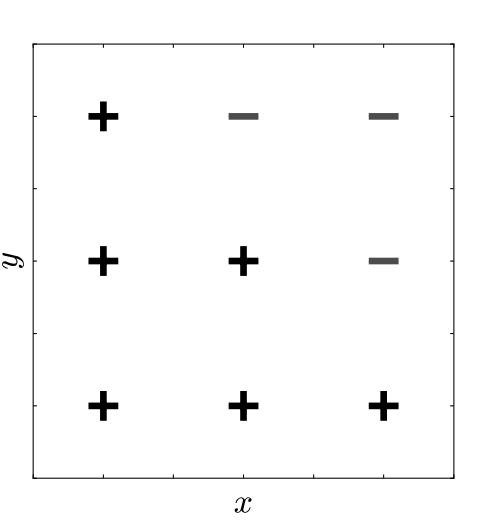
\includegraphics[width=0.28\linewidth,left]{images/2-1.png}
\end{figure}
\vspace{-5mm}
\item
اکنون فرض کنید که یادگیرنده‌های ضعیف ما درخت‌های تصمیم با عمق حداکثر 2 هستند، که خطای آموزشی وزن‌دار را کمینه می‌کنند. با استفاده از مجموعه داده‌ی زیر، مرز تصمیمی که توسط \(h_1\) یاد گرفته شده است را ترسیم کنید.
\begin{figure}[H]
    \latin
    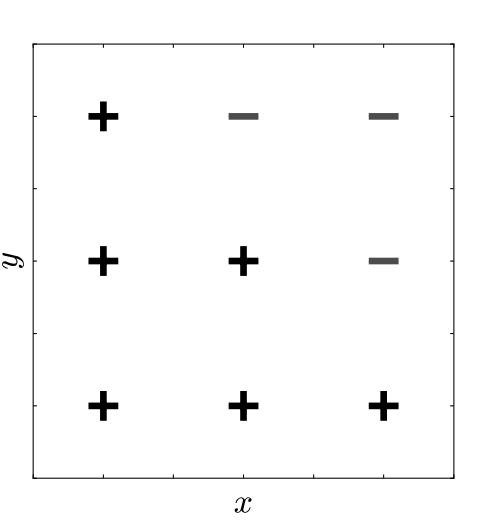
\includegraphics[width=0.28\linewidth,left]{images/2-1.png}
\end{figure}
\vspace{-5mm}
\item
 در مجموعه داده‌ی زیر، نقطه(ها) با بیشترین وزن در \lr{iteration} دوم را دایره بکشید و مرز تصمیمی که توسط \(h_2\) یاد گرفته شده است را ترسیم کنید.
\vspace{-5mm}
\begin{figure}[H]
    \latin
    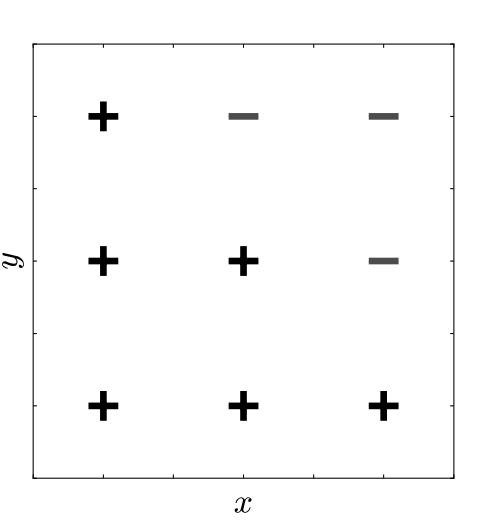
\includegraphics[width=0.28\linewidth,left]{images/2-1.png}
\end{figure}
\vspace{-5mm}
\item
در مجموعه داده‌ی زیر، مرز تصمیم \(H = \operatorname{sgn} (\alpha_1 h_1 + \alpha_2 h_2)\) را ترسیم کنید. (راهنمایی: نیازی به محاسبه صریح \(\alpha\) ها نیست).
\vspace{-5mm}
\begin{figure}[H]
    \latin
    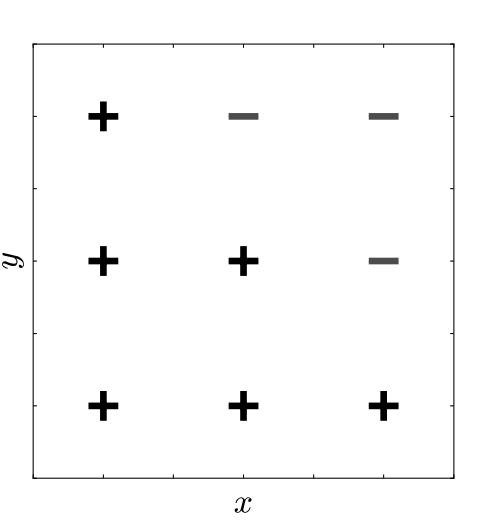
\includegraphics[width=0.28\linewidth,left]{images/2-1.png}
\end{figure}
\end{enumerate}
\pagebreak
    \textbf{پاسخ1:} 
    \begin{itemize}
        \item ابعاد فعال‌سازی: $126 \times 126 \times 64$
        \item تعداد پارامترها: $(3 \times 3 \times 3 + 1) \times 64 = 1792$
    \end{itemize}


        \textbf{پاسخ2:} 
    \begin{itemize}
        \item ابعاد فعال‌سازی: $128 \times 128 \times 16$
        \item تعداد پارامترها: $(5 \times 5 \times 3 + 1) \times 16 = 1216$
    \end{itemize}

        \textbf{پاسخ3:} 
    \begin{itemize}
        \item ابعاد فعال‌سازی: $64 \times 64 \times 32$
        \item تعداد پارامترها: $(2 \times 2 \times 3 + 1) \times 32 = 416$
    \end{itemize}


        \textbf{پاسخ4:} 
    \begin{itemize}
        \item ابعاد فعال‌سازی بعد از سه ماژول: $14 \times 14 \times 64$
        \item تعداد پارامترها: $(3 \times 3 \times 3 + 1) \times 64 + (3 \times 3 \times 64 + 1) \times 64 \times 2 = 75,648$
    \end{itemize}

    \textbf{پاسخ5:} 
    \begin{itemize}
        \item ابعاد فعال‌سازی بعد از سه ماژول: $16 \times 16 \times 16$
        \item تعداد پارامترها: $(5 \times 5 \times 3 + 1) \times 16 + (5 \times 5 \times 16 + 1) \times 16 \times 2 = 14,048$
    \end{itemize}



    
    \textbf{پاسخ6:} 
    \begin{itemize}
        \item ابعاد فعال‌سازی بعد از سه ماژول: $2 \times 2 \times 32$
        \item تعداد پارامترها: $(2 \times 2 \times 3 + 1) \times 32 + (2 \times 2 \times 32 + 1) \times 32 \times 2 = 8672$
    \end{itemize}

        \textbf{پاسخ7:} 
    \begin{itemize}
        \item کمترین تعداد پارامترها مربوط به معماری قسمت ۶ است، با ابعاد فعال‌سازی $2 \times 2 \times 32$.
        \item تعداد پارامترها: $(2 \times 2 \times 32 + 1) \times 10 = 1290$
    \end{itemize}
\pagebreak
\hrule
نام و نام خانوادگی: \hspace{8cm} شماره دانشجویی:
\hrule
\vspace{0.5cm}

\textbf{خوشه خوشه}

در این مسئله می‌خواهیم به بررسی الگوریتم خوشه بندی
k-means بپردازیم. فرض کنید \(X = {x_1, x_2, ..., x_n}\) داده‌های ما باشد و $\gamma$ یک ماتریس Indicator باشد به این صورت که $\gamma_{ij} = 1$ اگر \(x_i\) متعلق به خوشه j ام باشد و در غیر این صورت برابر ۰ است. فرض کنید $\mu_1, ..., \mu_k$ میانگین خوشه ها باشند. اعوجاج J برای داده‌ها به صورت زیر محاسبه می‌شود :
\[J(\gamma, \mu_1, ..., \mu_k) = n\sum_{j=1}^{k}\sum_{i=1}^{n}\gamma_{ij}\lVert x_i - \mu_j \rVert^2\]
همچنین \(C = 1, ..., k\) را به عنوان مجموعه خوشه ها در نظر بگیرید.
\begin{enumerate}
\item
آیا k-means نسبت به انتخاب نقاط اولیه حساس است، یعنی پاسخ آن بر اساس مجموعه‌ی نقاط اولیه تغییر می‌کند؟ اگر بله یک مثال ارائه کنید و اگر خیر، اثبات کنید.
\vspace{4cm}
\item
نشان دهید که الگوریتم k-means در زمان متناهی قدم به پایان می‌رسد. (راهنمایی: نشان دهید $J$ تعداد محدودی حالت دارد.)
\vspace{7cm}
\item
اگر ابعاد داده نسبت به تعداد نمونه‌ها خیلی زیاد باشد و عملا نمونه‌ها در یک فضای بزرگ پراکنده باشند، برای بهبود خوشه‌بندی از چه روشی استفاده می‌کنید؟
\pagebreak
\item
نشان دهید که کمینه J یک تابع غیرافزایشی بر حسب k یا همان تعداد خوشه هاست. در این صورت آیا انتخاب مقدار هایپرپارامتر $k$ بر اساس کمینه‌کردن مقداز $J$ ایده‌ی خوبی است؟ اگرنه، چه ایده‌ی بهتری دارید؟
\vspace{7cm}
\item
فرض کنید $\hat{x}$ میانگین داده‌های نمونه باشد. مقادیر زیر را در نظر بگیرید.
\[T(X) = \frac{\sum_{i=1}^{n}\lVert x_i - \hat{x}\rVert^2}{n}\]
\[W_j(X) = \frac{\sum_{i=1}^{n}\gamma_{ij}\lVert x_i - \mu_j\rVert^2}{\sum_{i=1}^{n}\gamma_{ij}}\]
\[B(X) = \sum_{j=1}^{k}\frac{\sum_{i=1}^{n}\gamma_{ij}}{n}\r\lVert \mu_j - \hat{x} \rVert^2\]
در اینجا \(T(X)\) نشان دهنده انحراف کلی، \(W_j(X)\) انحراف 
درون خوشه‌ای و \(B(X)\) انحراف بین خوشه‌ای است.
رابطه‌ی بین این ۳ مقدار به چه صورت است؟
نشان دهید که k-means میتواند به عنوان کمینه کننده میانگین وزن دار مقادیر درون خوشه‌ای و به طور تقریبی بیشینه کردن انحراف بین خوشه‌ای دیده شود.
\vspace{7cm}
\end{enumerate}
\pagebreak

آ) می‌توانیم مقادیر  را به صورت زیر بازنویسی کنیم:

\begin{align*}
& y_1 = \frac{x_1+x_2}{2} + \frac{|x_1-x_2|}{2} \\
& y_2 = \frac{x_1+x_2}{2} - \frac{|x_1-x_2|}{2}
\end{align*}

یعنی داریم:

$$
\rightarrow \begin{cases}
x_1 \ge x_2 \rightarrow \begin{cases} y_1 =  \frac{x_1+x_2}{2} + \frac{x_1-x_2}{2} = x_1 = \max(x_1, x_2) \\
y_2 = \frac{x_1+x_2}{2} - \frac{x_1 - x_2}{2} = x_2 = \min(x_1, x_2) \end{cases}\\

x_1 < x_2 \rightarrow \begin{cases} y_1 =  \frac{x_1+x_2}{2} - \frac{x_1-x_2}{2} = x_2 = \max(x_1, x_2) \\
y_2 = \frac{x_1+x_2}{2} + \frac{x_1 - x_2}{2} = x_1 = \min(x_1, x_2) \end{cases}
\end{cases}$$

در این صورت می‌توان گفت:

\begin{align*}
W^{(1)} &= \begin{bmatrix}1 & 1 \\ 1 & -1\end{bmatrix}
& b^{(1)} &= \begin{bmatrix}0 \\ 0\end{bmatrix}
& \phi^{(1)}(x) &= \begin{bmatrix}x_1 \\ |x_2|\end{bmatrix} \\
W^{(2)} &= \begin{bmatrix} 0.5 & 0.5 \\ 0.5 & -0.5\end{bmatrix}
&b^{(2)} &= \begin{bmatrix}0 \\ 0\end{bmatrix}
&\phi^{(2)}(x) &= \begin{bmatrix}x_1 \\ x_2\end{bmatrix}
\end{align*}

ب) با استفاده از ماژول پیاده‌سازی شده در بخش پیش داریم:

$$
\begin{bmatrix}
y_1 \\ y_2 \ \\ y_3 \ \\ y_4 \ 
\end{bmatrix} =
\begin{bmatrix}
\max \left(\max(x_1, x_2),~\max(x_3, x_4) \right)\\

\max \left(\min \left(\max(x_1, x_2),~\max(x_3, x_4) \right),~\max \left(\min(x_1, x_2),~\min(x_3, x_4) \right) \right)\\

\min \left(\min \left(\max(x_1, x_2),~\max(x_3, x_4) \right),~\max \left(\min(x_1, x_2),~\min(x_3, x_4) \right) \right)\\

\min \left(\min(x_1, x_2),~\min(x_3, x_4) \right)\\

\end{bmatrix} 
$$
\pagebreak
\hrule
نام و نام خانوادگی: \hspace{8cm} شماره دانشجویی:
\hrule
\vspace{0.5cm}
در هر بخش، درستی یا نادرستی گزینه را مشخص کرده و کامل توضیح دهید.
\begin{itemize}

    \item[الف)]
    در هنگام آموزش هرگونه مدل روی هر نوع مساله، از زمانی که تعداد پارامترها متناسب با تعداد ورودی‌ها شود به حداقل خطای تست می‌رسیم و پس از آن با افزایش تعداد پارامترها همیشه شاهد روند افزایشی خطای تست خواهیم بود.
    \item[ب)]
    معماری RNN سریع‌تر از Transformer است ولی دقت آن نسبت به Transformer کم‌تر است.

    \item[ج)]
    ابعاد فضای Embedding متن و تصویر در CLIP می‌تواند متفاوت باشد.
    
    \item[د)]
در یادگیری انتقالی با \lr{CNN}، زمانی که توزیع داده‌های هدف مشابه توزیع داده‌های پیش‌آموزش باشد، معمولاً چند لایه‌ی \lr{Fully Connected} آخر جایگزین شده و دوباره آموزش داده می‌شود، در حالی که وزن لایه‌های قبلی ثابت می‌مانند.

\item[ه)]
اگر یک مدل شبکه‌ی عصبی ۳ لایه برای رسیدن به دقت ۹۰ درصد روی یک مساله‌ی ورودی نیاز به ۱ میلیارد پارامتر داشته باشد، یک شبکه‌ی عصبی ۱۰ لایه برای رسیدن به همان سطح دقت روی همان مساله نیاز به تقریبا همان تعداد پارامتر دارد که البته عرض هر لایه کاهش می‌یابد.

\item[و)]
اگر از یک میلیارد تصویر داده شده، فقط یک میلیون تصویر برچسب داشته باشد برای خوشه‌بندی (Clustering) از کل یک میلیارد تصویر می‌توان استفاده کرد ولی برای دسته‌بندی (Classification) صرفا می‌توانیم از یک میلیون تصویر برچسب‌دار استفاده کنیم.
\item[ز)]
برای یک CNN با ابعاد کرنل $5\times 5$ و استراید ۱ و روی تصاویر $1000\times 1000$ داشتن سه لایه برای استخراج ویژگی‌های سراسری از تصویر کافی است.
\item[ح)]
استفاده از Patch ها به صورت انکد شده به عنوان ورودی ترانسفورمر ViT کافی نیست و حتما باید از 
\lr{Positional Embedding} استفاده کنیم.
\end{itemize}

\pagebreak
پاسخ سوال اینجا قرار خواهد گرفت.

\end{document}
